\chapter{Introduction}\label{ch:introduction}

Since the Industrial Revolution, the industry have been improving itself, increasing the number of machines in factories in order to intensify the production and to reduce the effort made by the workers. However, in the last few years, the industry motto have been changing, influenced by the development of the technology. The main goal is to try to decrease the number of people working in firms, reducing, thus, the cost with manpower, and increasing the number of autonomous machines. These mechanisms are able to work without breaks for long periods with a high level of accuracy. For instances, robot arms are one of the most used instruments in factories…


The Lego Group began manufacturing the lego bricks in 1949. 
Assume that you work in a company producing Simpson figures made by Dublo brucks.

\begin{enumerate}
	\item The figures come in two sizes. One size consisting of 3x1 (or 2x1 for Maggie) Dublo bricks and one consists of 3x4 (or 2x4 for Maggie) brick.
	\item A customer can order a set of figures
\end{enumerate}

The Dublo bricks are located randomly (but not
overlapping) on a table next to a robot.

\begin{enumerate}
	\item A camera is located above the table so that all the
	bricks are within the view of the camera.
	\item Your task is to design a system which can produce
	the Simpson figures. 
\end{enumerate}

\begin{figure}[hb]
  \centering
  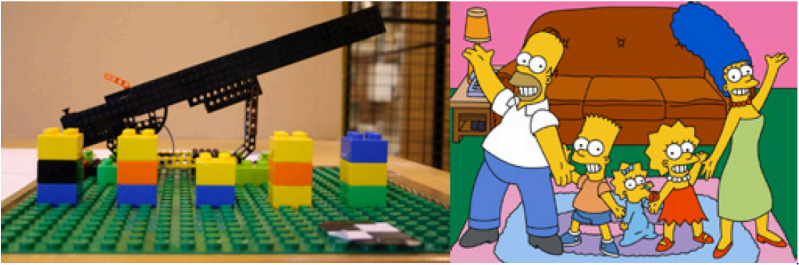
\includegraphics[width=4in]{figures/simpsonLegoBricks.png}
  \caption[Simpsons figures Lego Bricks] {A illustration of the simpsons figures with Lego Duplo Bricks}
\end{figure}

This involves among other things:
\begin{enumerate}
	\item Identifying which bricks are located on the table.
	\item Identifying the location of the bricks (e.g. the location of a
	black Dublo brick needed to build Homer)
	\item Determine the associated cost of each solution and the
	cheapest solutions.
	\item Grasping the bricks by means on a robot.
	\item Mounting the bricks on a plate or on top of other bricks
	\item Selecting the sequence in which you want to pick/place
	the bricks and build the figures
\end{enumerate}

\subsection*{Hardware}
\begin{enumerate}
	\item ADEPT Cobra
	\item Grapper
	\item Lego Blocks
	\item Logitech c920 HD Pro Webcam
\end{enumerate}

\subsection*{The Workspace} The ADEPT Cobra has to able to identify certain blocks inside its workspace. In order to so, a camera has been placed on the top of the cell where the robot is located, having a cenital point of view of the workspace.

The program will then perform an analysis of the picture in order to determine the color of the different blocks and their position in the workspace.
It is important to note that the scenario presented in this paper require different workspaces and frames.

First we have the 



